% --- Document: Preamble ---
\documentclass[../main.tex]{subfiles}
\graphicspath{{\subfix{../assets/}}}
% --- Document: Start ---
\begin{document}
% Sumário e lista de figuras
\tableofcontents
\listoffigures
\clearpage

% Cronogram
\section{Requisitos do Sistema}
Para definir e especificar bem o alcance do projeto, sua relevância e proposta, a investigação foi detalhada em requisitos funcionais e não funcionais, conforme as subseções delimitadas abaixo. 
%requisitos funcionais
\subsection{Requisitos Funcionais}
Os requisitos funcionais são todas as necessidades que devem ser atendidas pelo software por meio de serviços. Sendo eles no projeto: 
\vspace{3cm}
\begin{figure}[htbp]
    \centering
    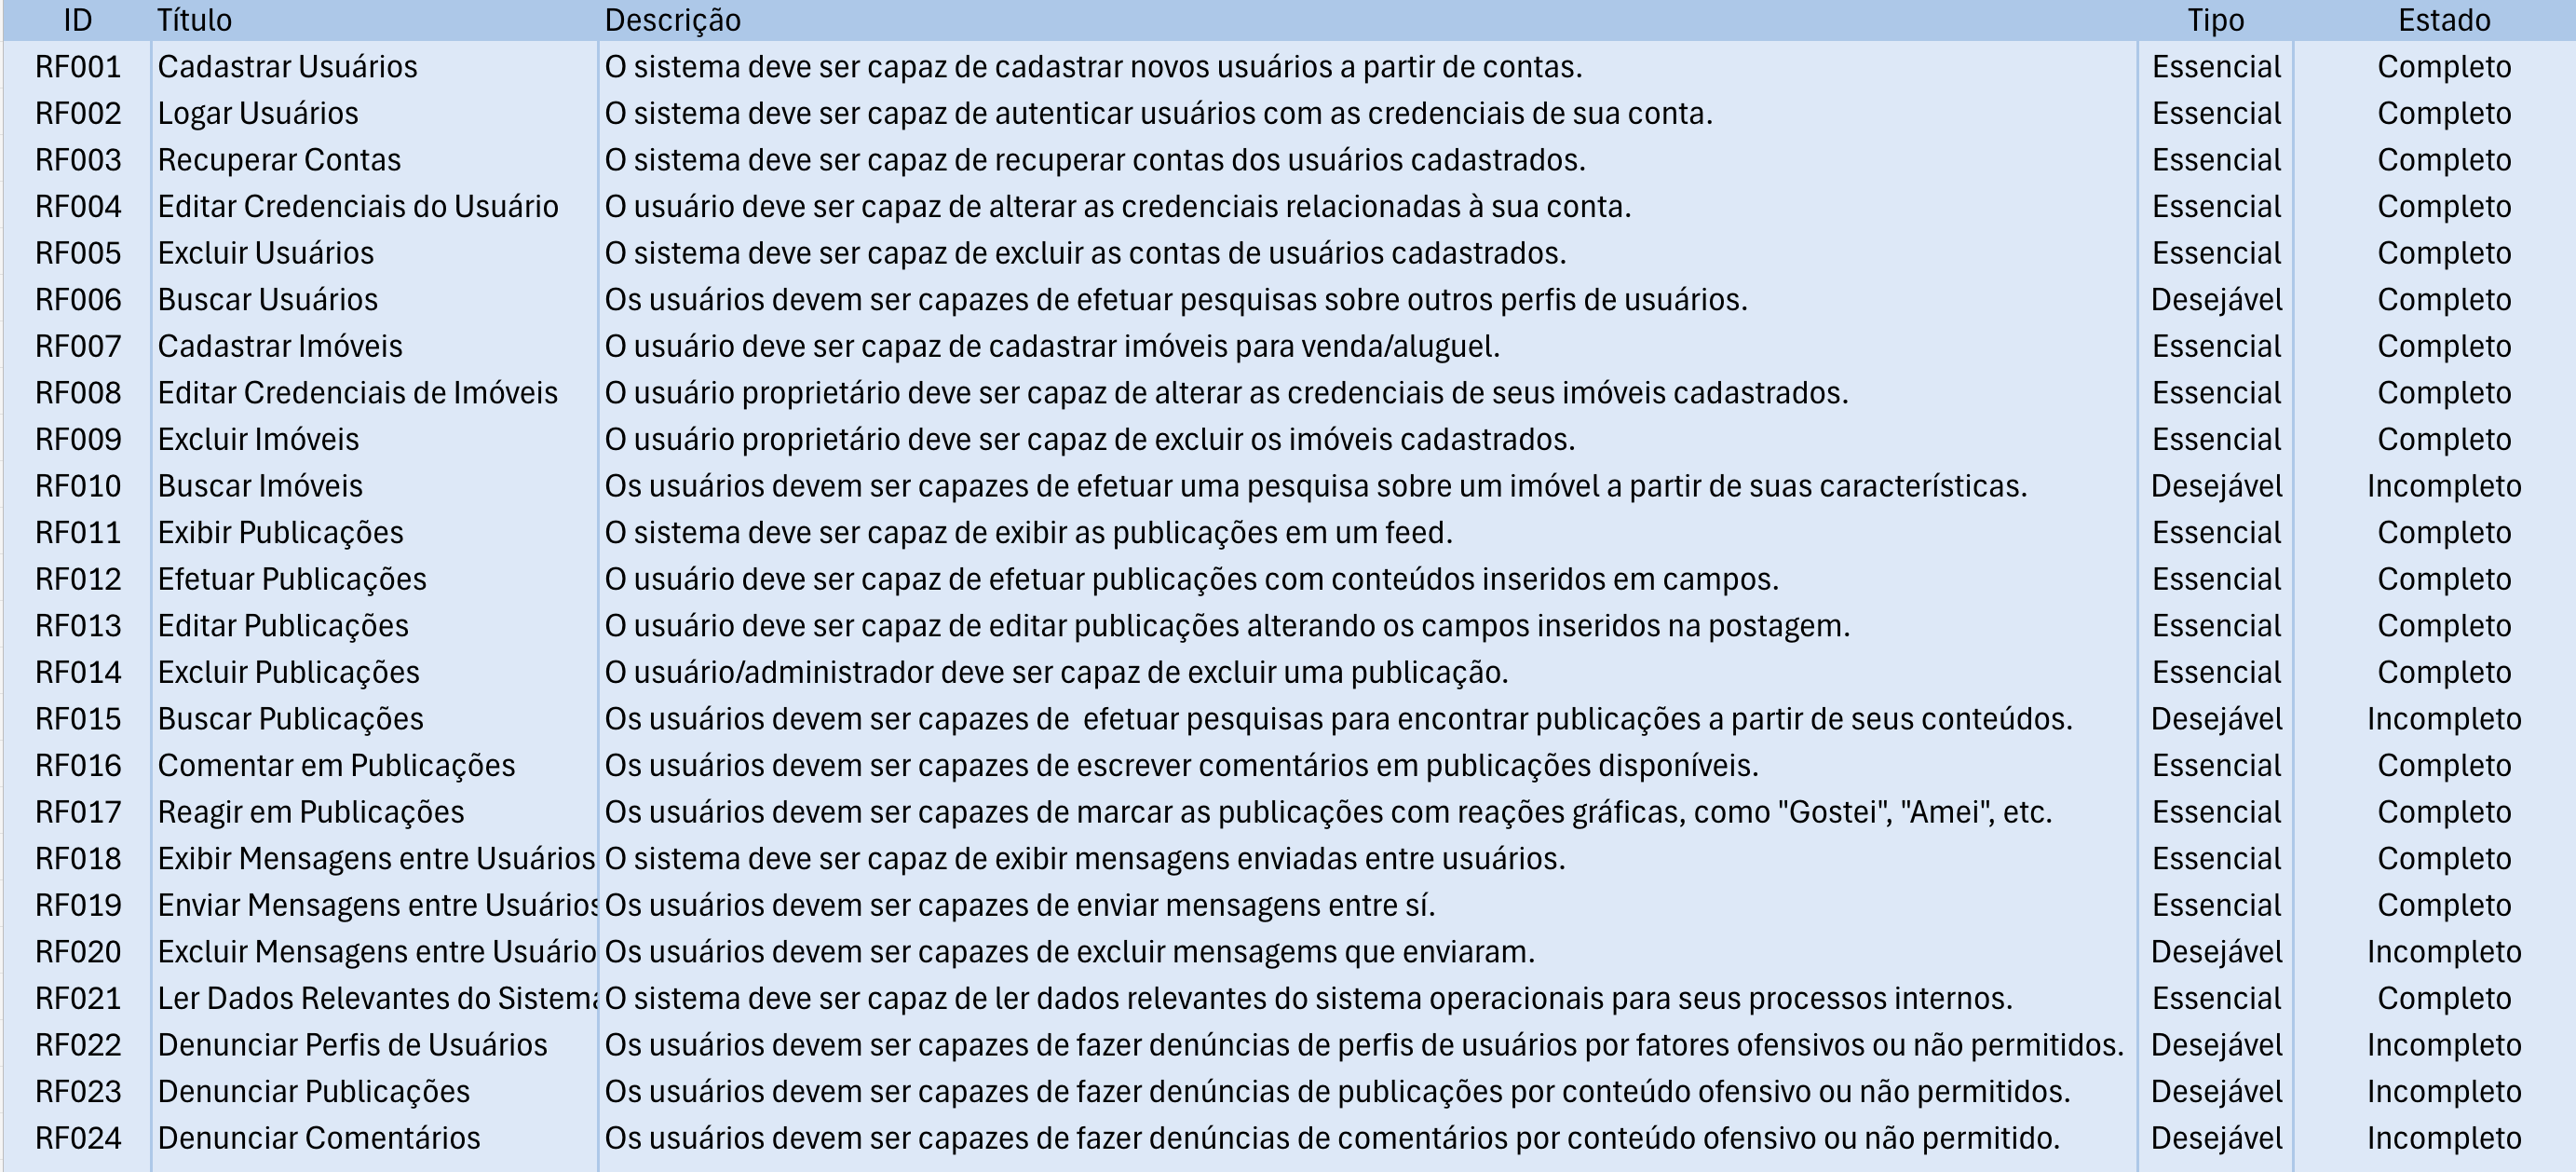
\includegraphics[width=0.8\textwidth]{diagrams/requisitosfuncionais.png}
    \caption{Diagrama dos Requisitos Funcionais}
    \label{fig:requisitos-funcionais}
\end{figure}
%requisitos nao funcionais
\subsection{Requisitos Não Funcionais}
Já os requisitos não funcionais são aqueles que descrevem como serão feitos os requisitos funcionais.
\vspace{3cm}
\begin{figure}[htbp]
    \centering
    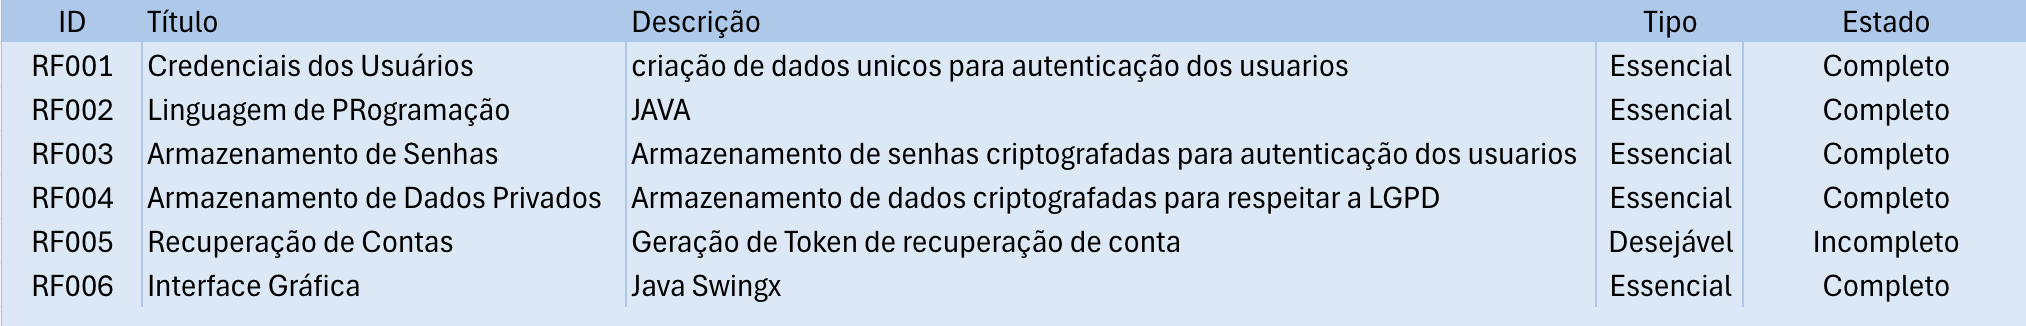
\includegraphics[width=0.8\textwidth]{diagrams/requisitosnaofuncionais.png}
    \caption{Diagrama dos Requisitos Não Funcionais}
    \label{fig:requisitos-nao-funcionais}
\end{figure}
\newpage
%Diagramas
\subsection{Diagramas UML}
\subsubsection{Casos de Uso}
Os casos de uso descrevem as interações entre os usuários (atores) e o sistema, detalhando como os usuários utilizarão o sistema para atingir seus objetivos. A seguir, apresentamos o diagrama de casos de uso, que ilustra visualmente essas interações:

\vspace{3cm}
\begin{figure}[htbp]
    \centering
    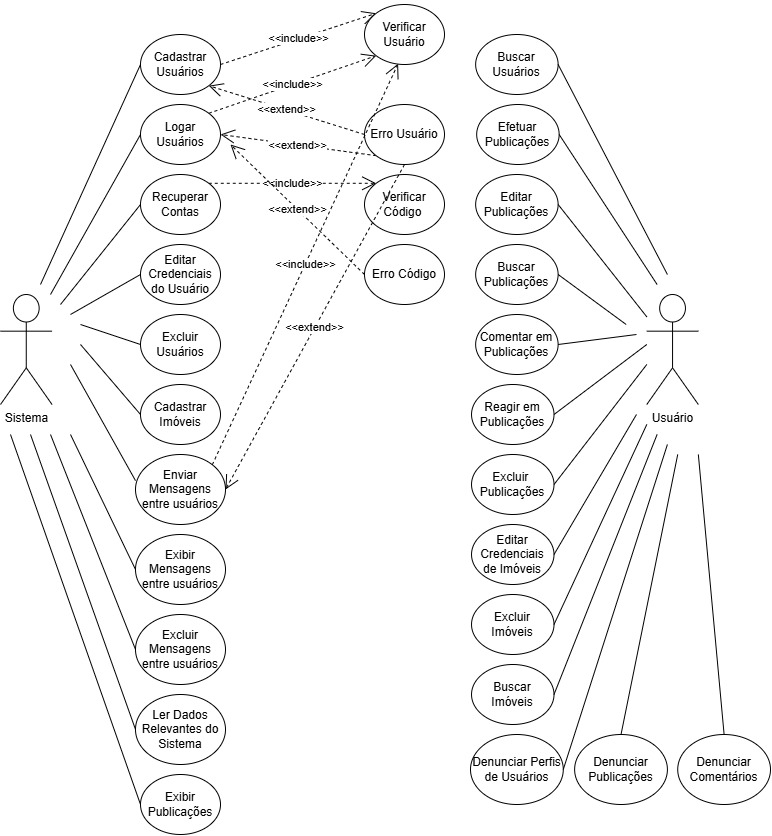
\includegraphics[width=0.8\textwidth]{diagrams/casosdeuso.jpg}
    \caption{Diagrama de Casos de Uso}
    \label{fig:casos-de-uso}
\end{figure}
\newpage
\subsubsection{Descrição dos Casos de Uso}
\begin{itemize}
    \item \textbf{Cadastro de Usuário}: Permite que novos usuários se registrem no sistema fornecendo informações obrigatórias e opcionais.
    \item \textbf{Login de Usuário}: Autentica os usuários já cadastrados, permitindo o acesso ao sistema.
    \item \textbf{Recuperação de Senha}: Permite que os usuários recuperem suas contas através da geração e verificação de um código.
    \item \textbf{Criação de Propriedades}: Permite que os usuários adicionem novas propriedades ao sistema.
    \item \textbf{Edição de Propriedades}: Permite que os usuários editem informações de propriedades existentes.
    \item \textbf{Remoção de Propriedades}: Permite que os usuários removam propriedades do sistema.
    \item \textbf{Criação de Postagens}: Permite que os usuários criem novas postagens.
    \item \textbf{Comentário em Postagens}: Permite que os usuários comentem em postagens existentes.
    \item \textbf{Chat entre Usuários}: Permite a comunicação entre usuários através de mensagens de chat.
\end{itemize}
\subsubsection{Descrição do Diagrama de Classes}
\begin{itemize}
    \item \textbf{Classe Usuário}: Representa um usuário do sistema, contendo atributos como nome, email, senha e métodos para autenticação e recuperação de conta.
    \item \textbf{Classe Propriedade}: Representa uma propriedade, contendo atributos como endereço, descrição e métodos para criação, edição e remoção.
    \item \textbf{Classe Postagem}: Representa uma postagem, contendo atributos como conteúdo, data de criação e métodos para criação e edição.
    \item \textbf{Classe Comentário}: Representa um comentário em uma postagem, contendo atributos como conteúdo e autor.
    \item \textbf{Classe Chat}: Representa o chat entre usuários, contendo atributos como mensagens e participantes.
\end{itemize}
%Class Diagram
\subsubsection{Classes}
O diagrama de classes representa a estrutura estática do sistema, mostrando as classes, seus atributos e métodos, além dos relacionamentos entre elas. A seguir, apresentamos o diagrama de classes do sistema:

\vspace{3cm}
\begin{figure}[htbp]
    \centering
    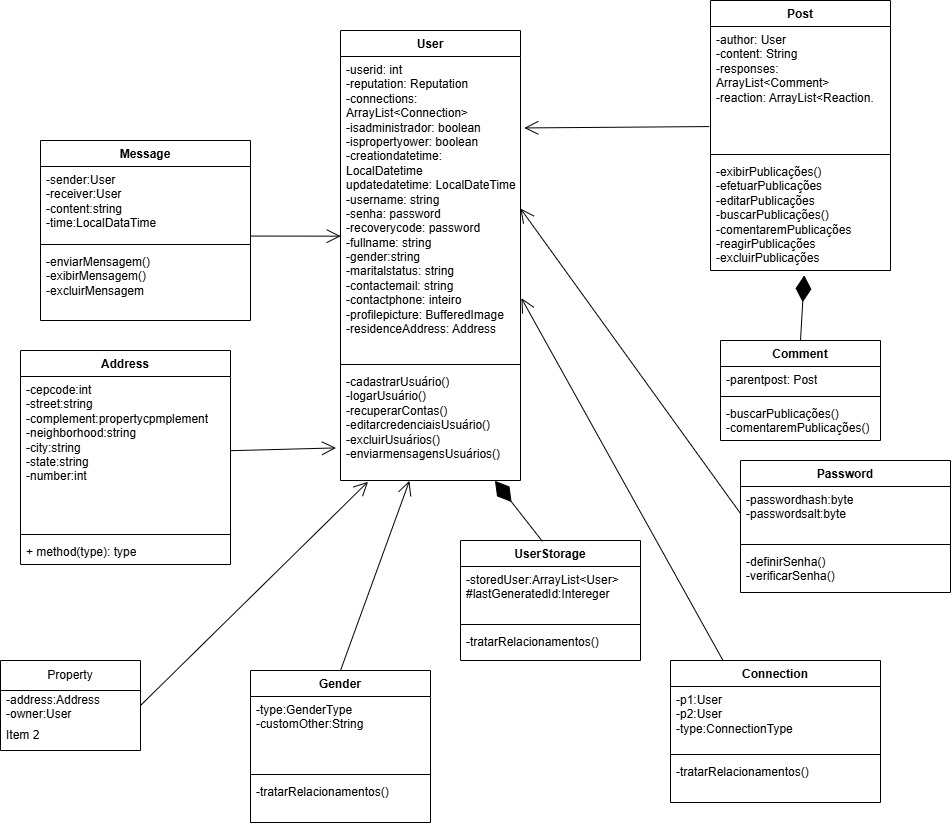
\includegraphics[width=0.8\textwidth]{diagrams/diagrama_de_classes.jpg}
    \caption{Diagrama de Classes}
    \label{fig:diagrama-de-classes}
\end{figure}
\newpage
%Sequence Diagram
\subsection{Diagrama de Sequência}
O diagrama de sequência mostra como os objetos interagem em um determinado caso de uso, detalhando a sequência de mensagens trocadas entre eles ao longo do tempo. A seguir, apresentamos o diagrama de sequência do sistema:

\vspace{3cm}
\begin{figure}[htbp]
    \centering
    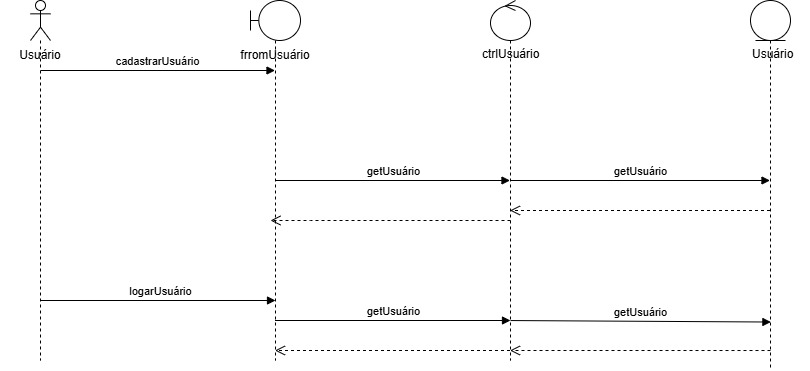
\includegraphics[width=0.8\textwidth]{diagrams/diagrama_de_sequencia.jpg}
    \caption{Diagrama de Sequência}
    \label{fig:diagrama-de-sequencia}
\end{figure}

\subsubsection{Descrição do Diagrama de Sequência}
\begin{itemize}
    \item \textbf{Cadastro de Usuário}: Detalha as interações entre o usuário e o sistema durante o processo de cadastro, incluindo a validação de dados e armazenamento das informações.
    \item \textbf{Login de Usuário}: Mostra a sequência de mensagens trocadas durante o processo de autenticação do usuário.
    \item \textbf{Criação de Propriedades}: Detalha os passos necessários para a criação de uma nova propriedade, desde a entrada dos dados até a confirmação do registro.
\end{itemize}


%Activity Diagram
\subsection{Diagrama de Atividade}
O diagrama de atividade representa o fluxo de atividades em um processo, mostrando as diferentes etapas e decisões que ocorrem ao longo do tempo. A seguir, apresentamos o diagrama de atividade do sistema:

\vspace{3cm}
\begin{figure}[htbp]
    \centering
    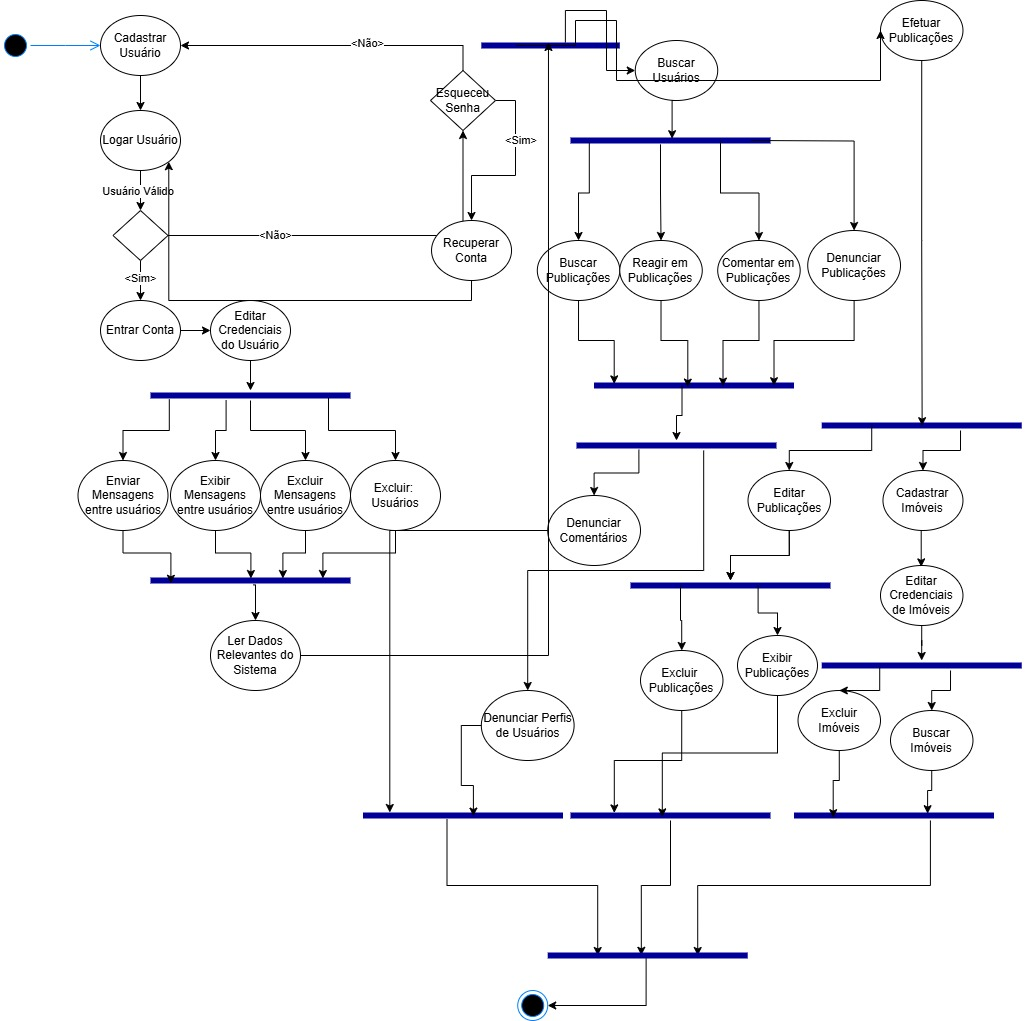
\includegraphics[width=0.8\textwidth]{diagrams/diagrama_de_atividade.jpg}
    \caption{Diagrama de Atividade}
    \label{fig:diagrama-de-atividade}
\end{figure}
\newpage
\subsubsection{Descrição do Diagrama de Atividade}
\begin{itemize}
    \item \textbf{Cadastro de Usuário}: Descreve o fluxo de atividades desde a entrada dos dados pelo usuário até a finalização do cadastro.
    \item \textbf{Login de Usuário}: Detalha as etapas do processo de autenticação, incluindo a verificação de credenciais e acesso ao sistema.
    \item \textbf{Criação de Postagem}: Mostra o fluxo de atividades envolvido na criação de uma nova postagem, desde a entrada do conteúdo até a publicação.
\end{itemize}
% --- Document: End ---
\end{document}

